%//==============================--@--==============================//%
\subsection[4.1 Diagrama de Bode e Relação Tempo-Frequência]{\hspace*{0.075 em}\raisebox{0.2 em}{$\pmb{\drsh}$} Diagrama de Bode e Relação Tempo-Frequência}
``The most useful technique for hand plotting was developed by H. W. Bode at Bell Laboratories between 1932 and 1942. The idea in Bode's method is to plot magnitude curves using a logarithmic scale and phase curves using a linear scale. This strategy allows us to plot a high-order $G(j\omega)$ by simply adding the separate terms graphically.
$$
    \frac{\bar{s}_1 \bar{s}_2}{\bar{s}_3 \bar{s}_4 \bar{s}_5} = \frac{r_1 e^{j\theta_1} r_2 e^{j\theta_2}}{r_3 e^{j\theta_3} r_4 e^{j\theta_4} r_5 e^{j\theta_5}} =
    \left( \frac{r_1 r_2}{r_3 r_4 r_5} \right) e^{j(\theta_1 + \theta_2 - \theta_3 - \theta_4 - \theta_5)}
$$
phases of the individual terms are added directly to obtain the phase of the composite expression, $G(j\omega)$. Furthermore, because
$$
    \vert G(j\omega) \vert = \frac{r_1 r_2}{r_3 r_4 r_5}
$$
it follows that
$$
    \log_{10}\vert G(j\omega) \vert = \log_{10}(r_1) + \log_{10}(r_2) - \log_{10}(r_3) - \log_{10}(r_4) - \log_{10}(r_5).\text{''\cite{FranklinPowell2015}}
$$

\begin{figure}[H]
    \centering
    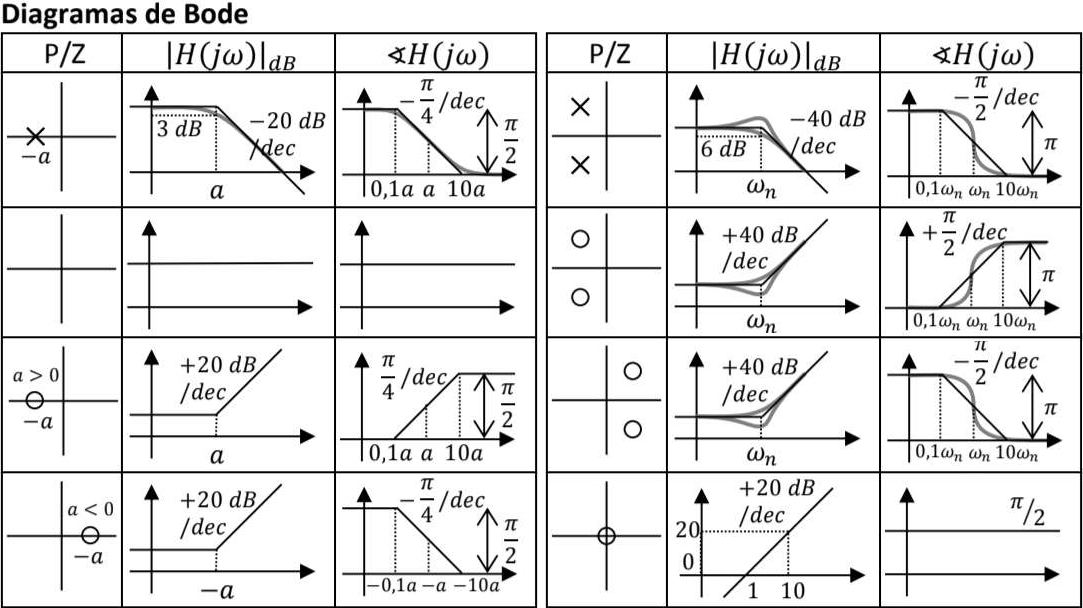
\includegraphics[width = 0.7\linewidth]{img/3/bode.png}
    \caption{Resposta assimtótica---resposta em diagramas de Bode.}
    \label{fig:bode}
\end{figure}

\noindent\textbf{Largura de banda} --- Banda de frequência na qual o módulo da função resposta em frequência não cai mais de 3dB em relação ao ganho de baixa frequência, traduz a capacidade de um sistema reproduzir mais ou menos perfeitamente os sinais aplicados à sua entrada.
%//==============================--@--==============================//%
\subsection[4.2 Critério de Nyquist]{\hspace*{0.075 em}\raisebox{0.2 em}{$\pmb{\drsh}$} Critério de Nyquist}

\noindent``The Nyquist stability criterion relates the open-loop frequency response to the number of closed-loop poles of the system in the RHP."\cite{FranklinPowell2015}

\vspace{1em}
\begin{itemize}
    \item Calcula a estabilidade do sistema em cadeia fechada sem avaliar explicitamente os pólos da f.t.c.f.
    \item Dá indicações sobre estabilidade relativa, através das margens de ganho e de fase.
\end{itemize}

\noindent Usa resultados da teoria das funções complexas (Teorema de Cauchy) para estudar a existência de zeros de $1+KG(s)H(s)$ no semi-plano complexo direito ou sobre o eixo imaginário.

%//==============================--@--==============================//%
\subsubsection[4.2.1 Teorema de Cauchy (Princípio do argumento)]{$\pmb{\rightarrow}$ Teorema de Cauchy (Princípio do argumento)}

{
\mdfsetup{linewidth=2pt}

\begin{mdframed}

    \begin{enumerate}
    \item Let $Z$ and $P$ be the number of zeros and poles of $L(s)$ inside $\Gamma$.
    \item As $s$ moves around $\Gamma$, $\angle L(s)$ undergoes a net change of $-(Z - P)2\pi$.
    \item A net change of $-2\pi$ means that the vector from $0$ to $L(s)$ swings clockwise around the origin one full rotation.
    \item A net change of $-(Z - P)2\pi$ means that the vector from $0$ to $L(s)$ must encircle the origin in a clockwise direction $(Z - P)$ times.
    \end{enumerate}

    \begin{theo}[\underline{Cauchy's Principle of the Argument}]{teo:cauchy}\label{teo:cauchy}
    Consider a transfer function $L(s)$ and a simple closed clockwise contour $\Gamma$. Let $Z$ and $P$ be the number of zeros and poles of $L(s)$ inside $\Gamma$.
    \begin{itemize}
    \item Then, the contour generated by evaluating $L(s)$ along $\Gamma$ will encircle the origin in a clockwise direction $Z - P$ times.
    \end{itemize}
    \end{theo}

    \begin{figure}[H]
        \centering
        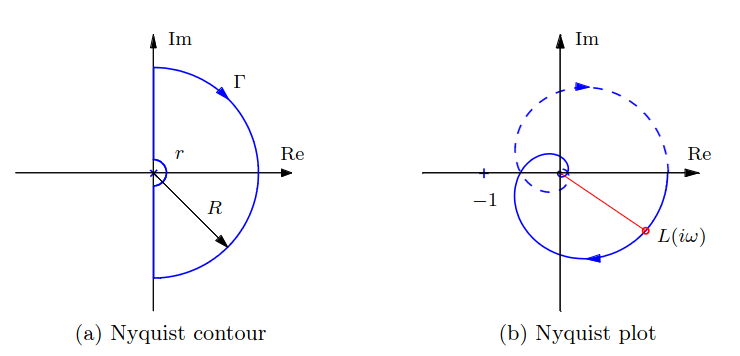
\includegraphics[width = 0.8\linewidth]{img/4/cauchy-arg-theorem.png}
        \label{fig:cauchy-theorem}
    \end{figure}
\end{mdframed}
}

A estabilidade em cadeia fechada é obtida se:
\begin{itemize}
    \item $N = 0$
    \item $Z = -P$
\end{itemize}

\noindent Assim, um sistema causal com f.t.c.a $KG(s)$ é estável em cadeia fechada sse

\begin{theo}[\underline{Critério de Nyquist}]{teo:Nyq}\label{teo:Nyq}
    Quando o afixo de s percorre o contorno de Nyquist num determinado sentido, o número de voltas que o afixo de $KG(s)$ percorre em torno do ponto –1 em sentido contrário é igual ao número de pólos da $KG(s)$ no interior do contorno de Nyquist.
\end{theo}

%//==============================--@--==============================//%